% impacto: memoria del proyecto (decision D-024).
% Compilar: pdflatex memoria.tex (dos veces, para el índice y el número de páginas).
% Las capturas van en figures/; las que faltan salen como un recuadro "Captura pendiente".

\documentclass[11pt,a4paper]{article}

\usepackage[T1]{fontenc}
\usepackage[spanish,es-tabla,es-nodecimaldot,es-noshorthands]{babel}
\usepackage{libertinus}
\usepackage{microtype}
\usepackage[a4paper,margin=2.5cm,headheight=14pt]{geometry}
\usepackage{graphicx}
\usepackage{xcolor}
\usepackage{booktabs}
\usepackage{tabularx}
\usepackage{array}
\usepackage{enumitem}
\usepackage{caption}
\usepackage{fancyhdr}
\usepackage{lastpage}
\usepackage{titlesec}
\usepackage{fancyvrb}
\usepackage[section]{placeins}
\usepackage{needspace}
\usepackage{tikz}
\usetikzlibrary{positioning,arrows.meta,fit,backgrounds}
\usepackage[hidelinks]{hyperref}

% ---- Colores: los mismos que la app (app/common.py) -------------------------------------------------
\definecolor{accent}{HTML}{6250D6}
\definecolor{accentlight}{HTML}{EFEDFB}
\definecolor{modelblue}{HTML}{2A78D6}
\definecolor{starsorange}{HTML}{EB6834}
\definecolor{badred}{HTML}{E34948}
\definecolor{ink}{HTML}{2B2A28}
\definecolor{muted}{HTML}{6F6E69}
\definecolor{rule}{HTML}{D9D8D2}

\hypersetup{
  colorlinks=true, linkcolor=ink, urlcolor=accent, citecolor=accent,
  pdftitle={impacto: memoria del proyecto},
  pdfauthor={Miguel Barranquero Diez},
  pdfsubject={Clasificación de reseñas con Neural Designer y OpenNN},
}

% ---- Tipografía de títulos, cabecera y pie ----------------------------------------------------------
\titleformat{\section}{\Large\sffamily\bfseries\color{ink}}{\color{accent}\thesection}{0.7em}{}
\titleformat{\subsection}{\large\sffamily\bfseries\color{ink}}{\color{accent}\thesubsection}{0.6em}{}
\titlespacing*{\section}{0pt}{2.2ex plus 1ex}{1.2ex}
\titlespacing*{\subsection}{0pt}{1.8ex plus 1ex}{0.8ex}

\pagestyle{fancy}
\fancyhf{}
\renewcommand{\headrulewidth}{0pt}
\fancyhead[L]{\small\sffamily\color{muted}impacto · Memoria del proyecto}
\fancyhead[R]{\small\sffamily\color{muted}\nouppercase{\rightmark}}
\fancyfoot[L]{\small\sffamily\color{muted}Miguel Barranquero Diez}
\fancyfoot[R]{\small\sffamily\color{muted}\thepage\ / \pageref*{LastPage}}
\renewcommand{\sectionmark}[1]{\markboth{#1}{#1}}
\renewcommand{\subsectionmark}[1]{}

\captionsetup{font=small, labelfont={bf,sf}, labelsep=period, justification=centering}
\setlist{itemsep=2pt, topsep=4pt}
\setlength{\parskip}{4pt}
\renewcommand{\arraystretch}{1.15}
\newcolumntype{R}{>{\raggedleft\arraybackslash}X}
\setcounter{tocdepth}{1}

% ---- Utilidades ----------------------------------------------------------------------------------
\newcommand{\pct}[1]{#1\,\%}
\newcommand{\code}[1]{\texttt{\small #1}}
% Captura de pantalla; si el archivo aún no existe, un recuadro con su nombre
\newcommand{\captura}[2][\linewidth]{%
  \IfFileExists{figures/#2}{\includegraphics[width=#1]{figures/#2}}{%
    \begin{tikzpicture}
      \node[draw=muted, dashed, rounded corners=4pt, minimum width=#1-2pt, minimum height=5cm,
            align=center, font=\sffamily\small, text=muted]
        {Captura pendiente\\[2pt]\texttt{figures/\detokenize{#2}}};
    \end{tikzpicture}}}
% Cifra destacada del resumen
\newcommand{\cifra}[2]{%
  \begin{minipage}[t]{0.235\linewidth}\centering
    {\fontsize{22}{24}\selectfont\sffamily\bfseries\color{accent}#1}\\[4pt]
    {\small\color{ink}#2}
  \end{minipage}}

\tikzset{
  caja/.style={draw=ink!70, rounded corners=3pt, align=center, font=\small\sffamily, fill=white,
               minimum height=1.15cm, text width=2.85cm, inner sep=4pt},
  clave/.style={caja, fill=accentlight, draw=accent},
  flecha/.style={-{Stealth[length=2.2mm]}, thick, color=ink!70},
  doble/.style={flecha, {Stealth[length=2.2mm]}-{Stealth[length=2.2mm]}},
  etiqueta/.style={font=\footnotesize\sffamily, text=muted},
}

\begin{document}

% =====================================================================================================
% Portada
% =====================================================================================================
\hypersetup{pageanchor=false}
\begin{titlepage}
  \newgeometry{margin=2.5cm}
  \setlength{\parindent}{0pt}
  \sffamily
  {\color{accent}\rule{\linewidth}{1.2pt}}\\[6pt]
  {\small\color{muted}MEMORIA DEL PROYECTO · MACHINE LEARNING DE EXTREMO A EXTREMO}

  \vspace{2.2cm}
  {\fontsize{48}{52}\selectfont\bfseries\color{ink}impacto}\\[10pt]
  {\LARGE\color{ink}Qué opinan los clientes de un negocio}\\[8pt]
  {\large\color{muted}Reseñas de Google clasificadas como buenas o malas con un modelo de texto
  entrenado en Neural Designer, ejecutado con OpenNN y desplegado con Docker}

  \vspace{1.4cm}
  \begin{center}
    \IfFileExists{figures/nd_network.png}
      {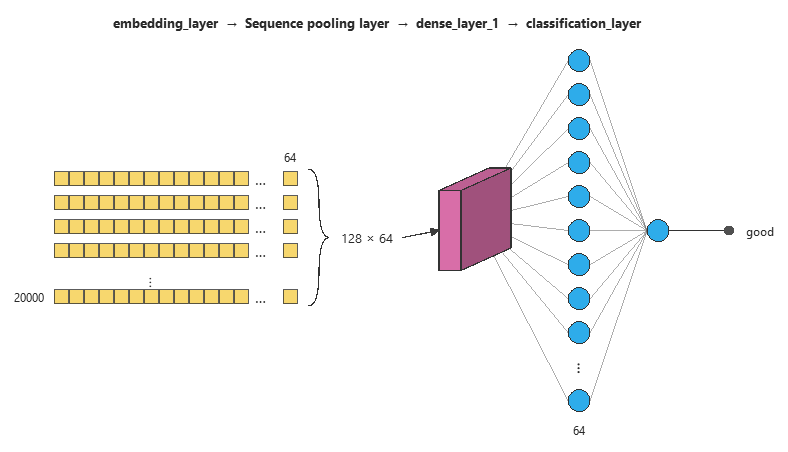
\includegraphics[width=\linewidth, height=8cm, keepaspectratio]{figures/nd_network.png}}
      {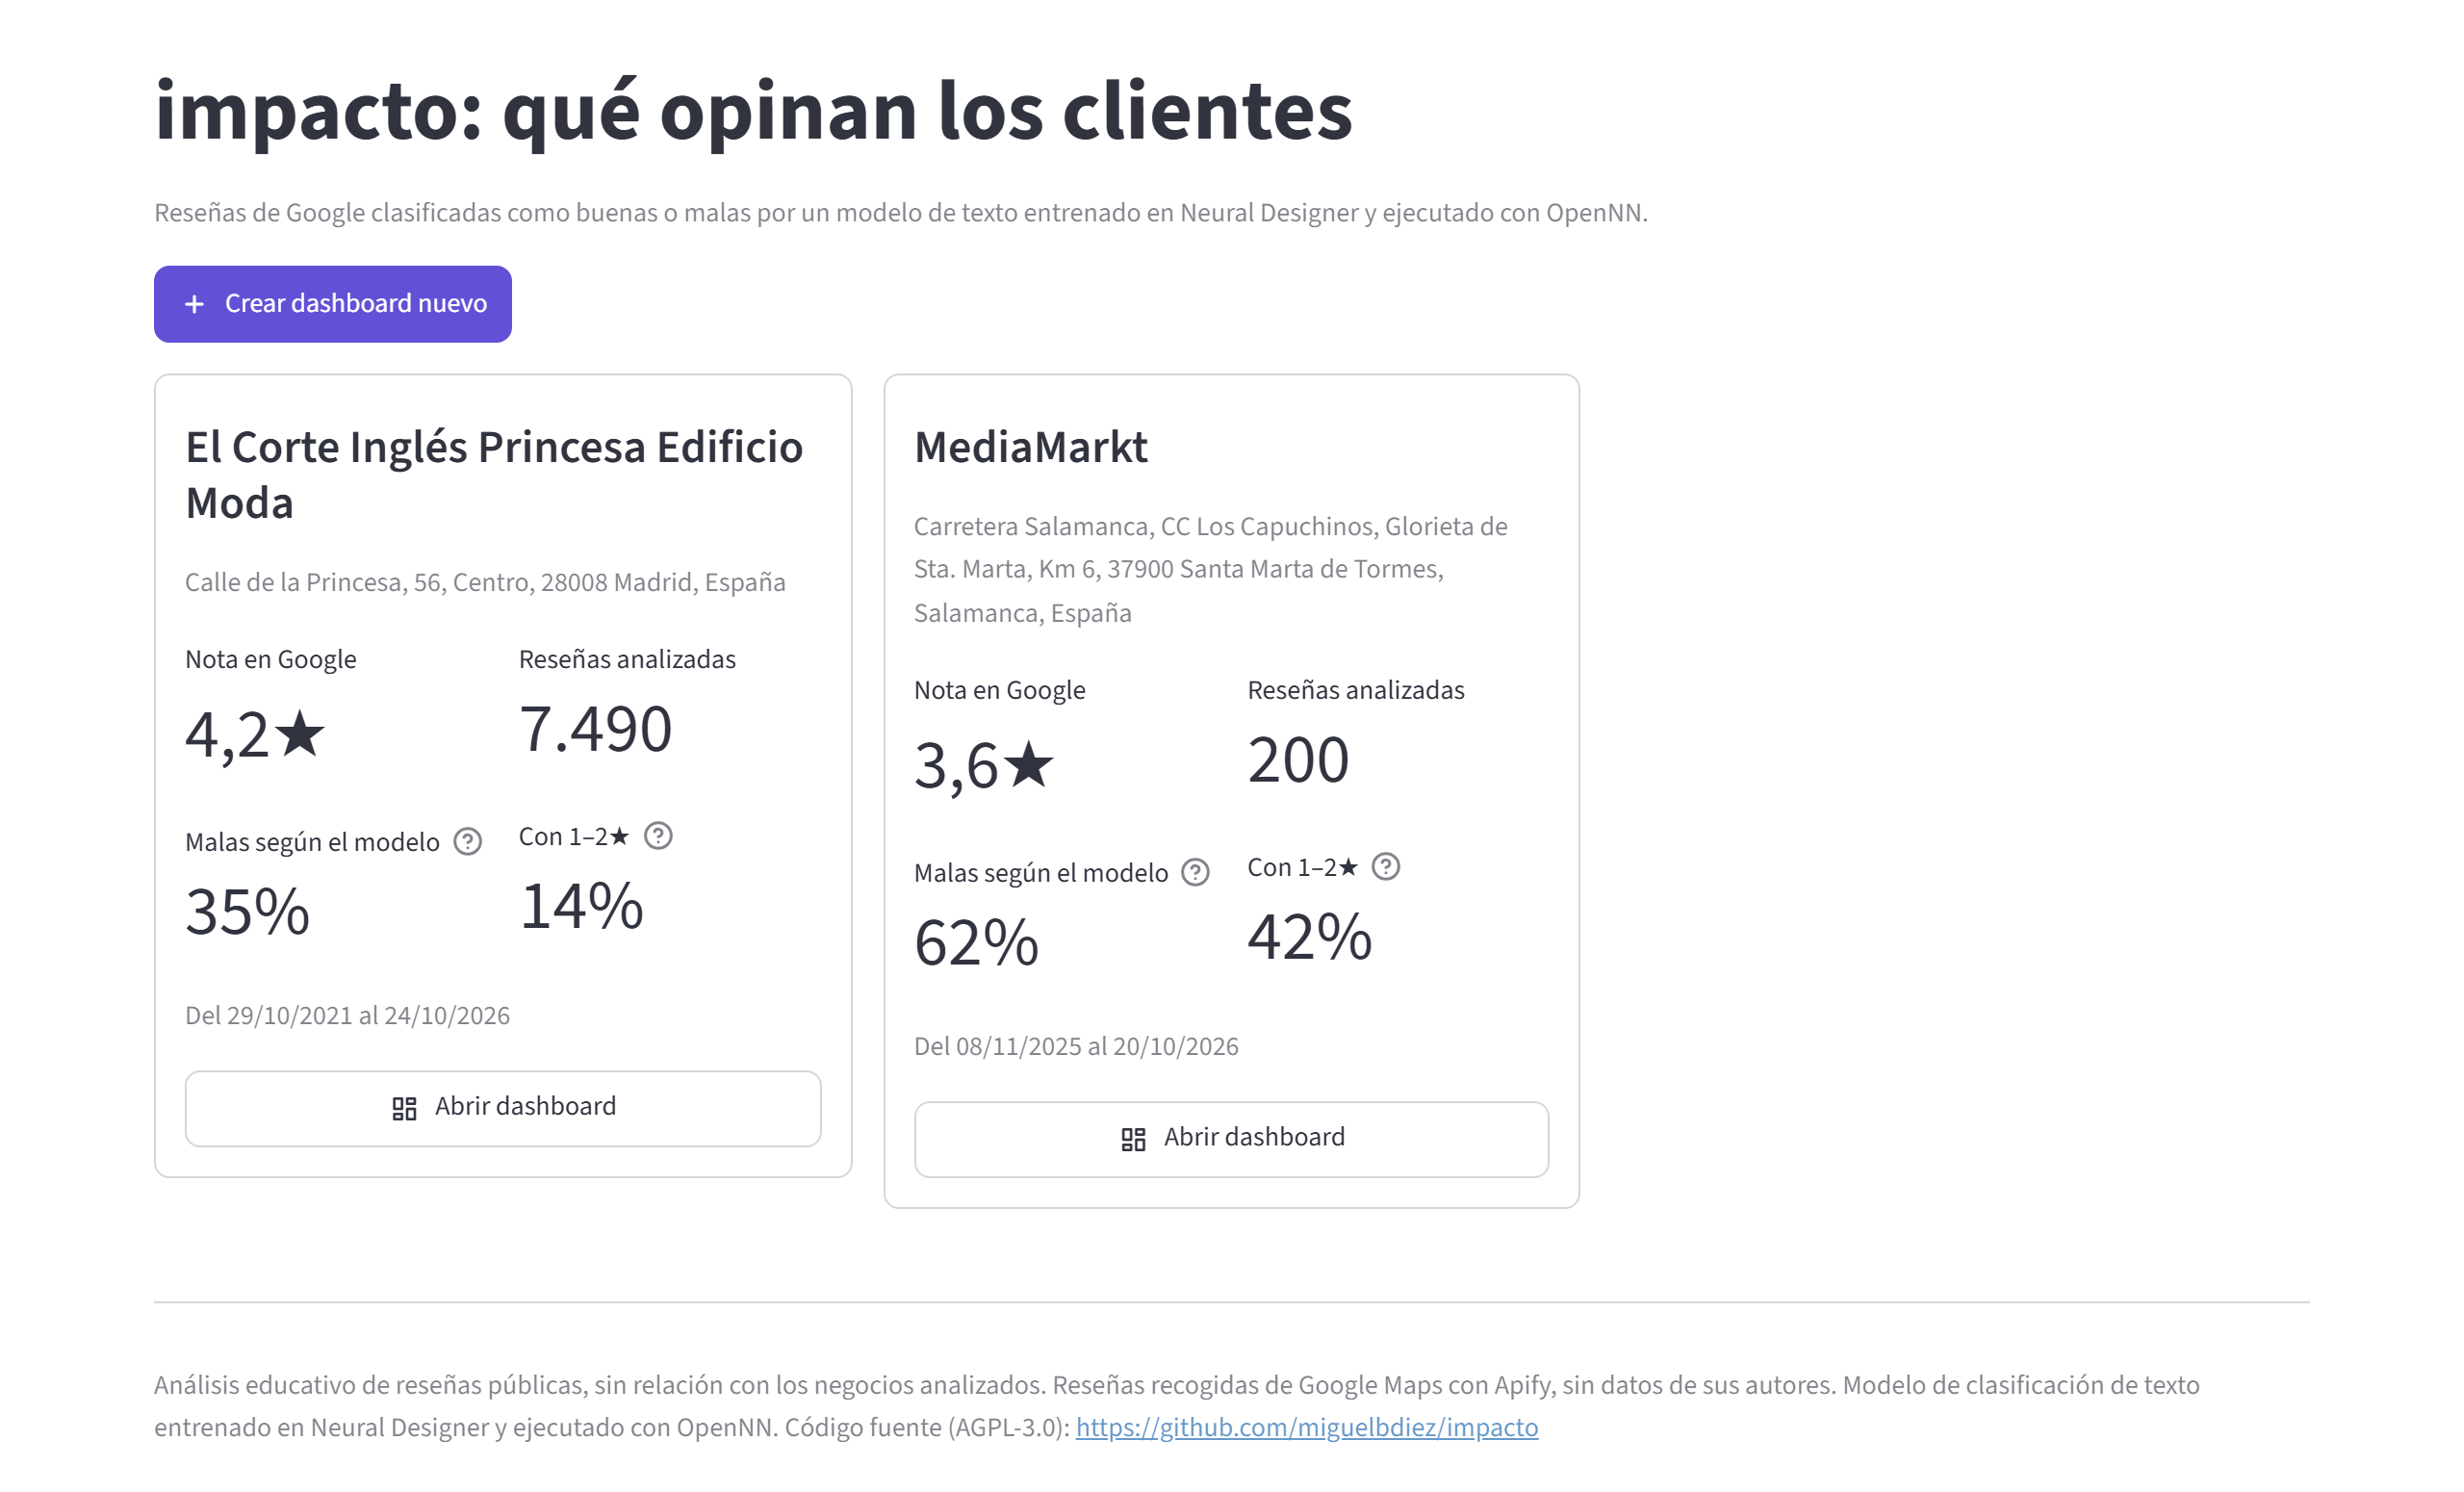
\includegraphics[width=0.92\linewidth]{figures/app_home.png}}
  \end{center}

  \vfill
  {\Large\bfseries\color{ink}Miguel Barranquero Diez}\\[6pt]
  {\small
  \begin{tabular}{@{}l@{\hspace{8pt}}l@{}}
    \color{muted}GitHub   & \href{https://github.com/miguelbdiez}{github.com/miguelbdiez} \\
    \color{muted}Código   & \href{https://github.com/miguelbdiez/impacto}{github.com/miguelbdiez/impacto} \\
    \color{muted}LinkedIn & \href{https://www.linkedin.com/in/miguel-barranquero-diez}{linkedin.com/in/miguel-barranquero-diez} \\
  \end{tabular}}

  \vspace{0.8cm}
  {\color{accent}\rule{\linewidth}{1.2pt}}\\[4pt]
  {\small\color{muted}Octubre de 2026}
  \restoregeometry
\end{titlepage}
\hypersetup{pageanchor=true}

% =====================================================================================================
% Resumen e índice
% =====================================================================================================
\section*{Resumen}
\markboth{Resumen}{Resumen}

\textbf{impacto} recoge las reseñas públicas de Google de un negocio, clasifica cada una como buena o mala con un
modelo de texto en español y muestra los resultados en una aplicación web y en un informe de Power BI: cómo
evolucionan las opiniones, si el modelo coincide con las estrellas y de qué hablan las reseñas malas y las buenas.

El modelo se entrenó en \textbf{Neural Designer} con 80.000 reseñas de Amazon en español y se ejecuta con un
pequeño programa en C++ basado en \textbf{OpenNN}, sin el motor completo de la aplicación. El caso de estudio son
7.490 reseñas de El Corte Inglés Princesa (Madrid) publicadas entre octubre de 2021 y octubre de 2026. Todo el
sistema, con la base de datos PostgreSQL, arranca con un solo comando de Docker. El proyecto no ha costado nada:
solo se han usado herramientas libres y planes gratuitos.

\vspace{10pt}
\noindent
\cifra{\pct{88,5}}{exactitud en reseñas que el modelo no había visto}\hfill
\cifra{\pct{87,1}}{coincidencia con las estrellas en reseñas reales}\hfill
\cifra{7.490}{reseñas de Google analizadas}\hfill
\cifra{0\,€}{de coste, solo planes gratuitos}
\vspace{14pt}

\noindent{\color{rule}\rule{\linewidth}{0.6pt}}
\vspace{-14pt}
\renewcommand{\contentsname}{\normalsize\sffamily\bfseries Contenido}
{\small\tableofcontents}

\newpage

% =====================================================================================================
\section{Introducción y objetivos}
% =====================================================================================================

\subsection{Motivación}

La nota media de Google resume en un número miles de opiniones, pero no dice qué está cambiando ni por qué. Un
negocio con 4,2 estrellas puede tener cada año más clientes descontentos sin que la media apenas se mueva. Leer las
reseñas una a una no escala.

Este proyecto clasifica el \emph{texto} de cada reseña con un modelo de aprendizaje automático. Las estrellas ya
existen, pero el modelo de texto sirve para algo más: en el futuro podrá clasificar opiniones que no llevan
estrellas, como mensajes de foros o de redes sociales. Mientras tanto, las estrellas de Google sirven para
comprobar gratis si el modelo acierta en un dominio real.

Es un proyecto de portfolio y recorre el ciclo completo: datos de entrenamiento, entrenamiento y evaluación del
modelo, despliegue de la inferencia, recogida de datos reales, almacenamiento, análisis, visualización y
despliegue. El modelo se entrenó en Neural Designer, la aplicación de machine learning de Artelnics en cuyo
desarrollo trabaja el autor, de modo que el proyecto sirve también como caso práctico de la herramienta.

\subsection{Objetivos}

\begin{enumerate}
  \item Entrenar en Neural Designer un clasificador de texto en español (\emph{buena} / \emph{mala}) y compararlo
        con un modelo de referencia clásico.
  \item Ejecutar el modelo fuera de Neural Designer con un programa ligero basado en OpenNN, con los mismos
        resultados.
  \item Recoger las reseñas de un negocio real sin coste y sin datos personales de sus autores.
  \item Analizar los resultados: evolución en el tiempo, coincidencia con las estrellas y temas de las reseñas.
  \item Mostrarlos en una aplicación web (Streamlit) y en un informe de Power BI.
  \item Desplegarlo todo con Docker.
  \item Documentar cada decisión, con las alternativas y los motivos, en un registro de decisiones.
\end{enumerate}

\subsection{Caso de estudio y restricciones}

El caso de estudio es \textbf{El Corte Inglés Princesa (Edificio Moda)}, en la calle de la Princesa de Madrid:
4,2 estrellas y 13.706 reseñas en Google. Una marca conocida a nivel nacional hace el resultado más cercano, y su
número de reseñas cabe en el plan gratuito del servicio de recogida (El Corte Inglés de Castellana, con más de
42.000, se descartó por eso). La aplicación permite analizar cualquier otro negocio.

\emph{Este es un análisis educativo de reseñas públicas, sin relación con la empresa. Se muestran cifras
agregadas y fragmentos cortos, nunca el conjunto de los textos.}

Tres restricciones han guiado el diseño:
\begin{itemize}
  \item \textbf{Coste cero.} Solo herramientas libres y planes gratuitos, sin ningún medio de pago registrado.
  \item \textbf{Privacidad.} No se guardan nombres, fotos ni perfiles de los autores de las reseñas, y nunca se
        evitan CAPTCHAs ni bloqueos.
  \item \textbf{Licencias de datos.} Los datos de entrenamiento no se pueden redistribuir: el repositorio incluye
        los scripts que los reconstruyen, no los datos.
\end{itemize}

% =====================================================================================================
\section{Arquitectura y tecnologías}
% =====================================================================================================

El sistema tiene dos partes (figura~\ref{fig:pipeline}). El \textbf{entrenamiento} se hace una vez: reseñas de
Amazon, normalización del texto y entrenamiento en Neural Designer, de donde se exporta la red. La
\textbf{producción} se repite con cada negocio: descarga de reseñas de Google Maps, base de datos, clasificación con
el predictor de OpenNN y visualización.

\begin{figure}[htbp]
\centering
\begin{tikzpicture}[node distance=0.55cm and 0.95cm, caja/.append style={text width=2.5cm}]
  % Entrenamiento
  \node[caja] (amazon) {Reseñas de Amazon\\en español\\\footnotesize 80.000 reseñas};
  \node[caja, right=of amazon] (norm) {Normalización\\a ASCII\\\footnotesize\texttt{text.py}};
  \node[clave, right=of norm] (nd) {\textbf{Neural Designer}\\entrenamiento\\y evaluación};
  \node[caja, right=of nd] (export) {Exportación\\\footnotesize red, pesos\\y vocabulario};
  % Producción
  \node[caja, below=1.4cm of amazon] (maps) {Google Maps\\\footnotesize reseñas públicas};
  \node[caja, right=of maps] (json) {Descargas JSON\\\footnotesize sin datos\\de los autores};
  \node[caja, right=of json] (db) {Base de datos\\\footnotesize SQLite / PostgreSQL};
  \node[clave, right=of db] (pred) {\textbf{Predictor OpenNN}\\\footnotesize C++ · CPU};
  % Salidas
  \node[caja, below=1.1cm of json] (app) {App web\\\footnotesize Streamlit};
  \node[caja, below=1.1cm of pred] (pbi) {Informe\\\footnotesize Power BI};

  \draw[flecha] (amazon) -- (norm);
  \draw[flecha] (norm) -- (nd);
  \draw[flecha] (nd) -- (export);
  \draw[flecha] (export) -- (pred);
  \draw[flecha] (maps) -- node[above, etiqueta] {Apify} (json);
  \draw[flecha] (json) -- (db);
  \draw[flecha] ([yshift=5pt]db.east) -- node[above, etiqueta] {textos} ([yshift=5pt]pred.west);
  \draw[flecha] ([yshift=-5pt]pred.west) -- node[below, etiqueta] {predicción} ([yshift=-5pt]db.east);
  \draw[flecha] (db.south) -- ++(0,-0.45) -| (app.north);
  \draw[flecha] (db.south) -- ++(0,-0.45) -| (pbi.north);

  \node[etiqueta, anchor=south west] at ([yshift=4pt]amazon.north west) {ENTRENAMIENTO (UNA VEZ)};
  \node[etiqueta, anchor=south west] at ([yshift=4pt]maps.north west) {PRODUCCIÓN (CADA NEGOCIO)};
\end{tikzpicture}
\caption{Arquitectura de impacto. En violeta, las dos piezas del modelo: Neural Designer para entrenar y OpenNN
para predecir.}
\label{fig:pipeline}
\end{figure}

\begin{table}[htbp]
\centering\small
\caption{Tecnologías utilizadas.}
\label{tab:tecnologias}
\begin{tabularx}{\linewidth}{@{}>{\bfseries}l l X@{}}
\toprule
Etapa & Tecnología & Uso \\
\midrule
Datos            & Python, pandas, Hugging Face        & Descarga y preparación de las reseñas de entrenamiento \\
Entrenamiento    & Neural Designer                     & Red neuronal, entrenamiento, informes y matriz de confusión \\
Referencia       & scikit-learn                        & Modelo clásico TF-IDF con regresión logística, para comparar \\
Inferencia       & OpenNN (C++20), CMake               & Predictor ligero que ejecuta la red exportada \\
Recogida         & Apify (plan gratuito), Playwright   & Descarga de reseñas de Google Maps y búsqueda de negocios \\
Almacenamiento   & SQLAlchemy, SQLite, PostgreSQL 17   & Reseñas, descargas y predicciones \\
Visualización    & Streamlit, Altair, Power BI Desktop & Aplicación web, gráficos e informe con DAX y DirectQuery \\
Despliegue       & Docker, Docker Compose              & Aplicación y base de datos en contenedores \\
Entorno          & uv, Git, GitHub                     & Dependencias reproducibles y control de versiones \\
\bottomrule
\end{tabularx}
\end{table}

\paragraph{Registro de decisiones.} Todas las decisiones del proyecto están documentadas, con su contexto, las
alternativas consideradas y los motivos, en el archivo \code{docs/decision-log.md} del repositorio. Cuando una decisión
cambió, se añadió una actualización con fecha en lugar de reescribirla. Esta memoria resume ese registro.

% =====================================================================================================
\section{Datos de entrenamiento}
% =====================================================================================================

\subsection{El conjunto de datos}

Un solo negocio no tiene reseñas suficientes para entrenar un modelo, y casi todas son de 4 y 5 estrellas. Por eso el
modelo se entrena con un conjunto público: la parte en español del \emph{Multilingual Amazon Reviews
Corpus}~\cite{keung2020}, con 200.000 reseñas de productos repartidas por igual entre 1 y 5 estrellas. Su licencia
permite el uso no comercial y prohíbe redistribuir los datos, así que el repositorio documenta la fuente, cada paso
de procesado y las sumas de comprobación, e incluye los scripts que reconstruyen los archivos.

\subsection{De estrellas a etiquetas: dos clases}

Las estrellas dan la etiqueta: 1--2 estrellas, \emph{mala}; 4--5, \emph{buena}. Las de 3 estrellas se descartan.

Antes se probó una tercera clase, \emph{neutra}, para las de 3 estrellas. Las redes llegaron al \pct{62,8} de
exactitud y el modelo de referencia al \pct{65,8}--\pct{68,0}. Casi todos los errores estaban en la clase neutra:
solo se reconocía entre el \pct{49} y el \pct{56} de las reseñas neutras, mientras que confundir una buena con una
mala ocurría en el \pct{4}--\pct{9} de los casos. Una reseña de 3 estrellas mezcla elogios y quejas, así que las
estrellas dan una etiqueta fiable para los extremos y ruidosa para el centro. El modelo final usa dos clases, con
40.000 reseñas de cada una.

Solo el texto de la reseña es entrada del modelo. El título no se usa, porque las reseñas de Google y los mensajes
de redes sociales no lo tienen, y las estrellas tampoco, porque de ellas sale la etiqueta.

\subsection{Un problema con los acentos}

El vocabulario del primer modelo tenía entre sus palabras más frecuentes fragmentos como \code{m}, \code{s},
\code{est} o \code{peque}. La causa estaba en el tokenizador de palabras de OpenNN: clasifica el texto byte a byte,
y en UTF-8 las letras con tilde, la ñ y los signos ¿ ¡ ocupan dos bytes que no cuentan como letras. La palabra se
partía en dos (tabla~\ref{tab:tokens}). Afectaba al \pct{7,5} de las palabras del conjunto de datos.

\begin{table}[htbp]
\centering\small
\caption{Cómo partía las palabras el tokenizador de OpenNN antes de normalizar el texto.}
\label{tab:tokens}
\begin{tabular}{@{}ll@{\hspace{1.5cm}}ll@{}}
\toprule
Texto & Tokens & Texto & Tokens \\
\midrule
más     & \code{m}, \code{s}       & también & \code{tambi}, \code{n} \\
pequeño & \code{peque}, \code{o}   & mañana  & \code{ma}, \code{ana} \\
\bottomrule
\end{tabular}
\end{table}

La solución fue normalizar el texto a ASCII (\emph{más} pasa a \emph{mas}) en una única función,
\code{normalize\_text}, que usan tanto la preparación de los datos de entrenamiento como la inferencia. Así el modelo
ve exactamente los mismos tokens al entrenar y al predecir. Se pierden distinciones como \emph{año}/\emph{ano}, que
no importan para el sentimiento. El arreglo de fondo, un tokenizador que entienda UTF-8, se comunicó al equipo de
OpenNN.

% =====================================================================================================
\section{Entrenamiento con Neural Designer}
% =====================================================================================================

\subsection{Configuración}

El archivo de entrenamiento se cargó en un proyecto de clasificación de texto de Neural Designer. Cada columna recibe
un papel: el texto es la entrada, la etiqueta es el objetivo y el resto de columnas (identificadores, categoría del
producto, estrellas, título) no se usan. Los datos se dividen en \pct{60} para entrenamiento, \pct{20} para
validación (Neural Designer lo llama \emph{selección}) y \pct{20} para prueba: 48.000, 16.000 y 16.000 reseñas.

\begin{itemize}
  \item \textbf{Vocabulario:} palabras que aparecen al menos dos veces, hasta 20.000. Las que aparecen una sola vez
        son sobre todo erratas.
  \item \textbf{Longitud de secuencia:} 128 tokens. La reseña mediana tiene 28 y el \pct{98,6} cabe en 128.
\end{itemize}

\subsection{Arquitectura de la red}

La red seleccionada (figura~\ref{fig:nd-red}) es sencilla:

\begin{enumerate}
  \item \textbf{Embedding} de 20.000 palabras en 64 dimensiones, con codificación posicional.
  \item \textbf{Average pooling:} la media de los vectores de la reseña, ignorando el relleno.
  \item \textbf{Capa densa} de 64 neuronas con activación ReLU.
  \item \textbf{Salida sigmoide:} la probabilidad de que la reseña sea buena.
\end{enumerate}

Tiene 1.284.225 parámetros, casi todos en la tabla de embedding.

\begin{figure}[htbp]
\centering
\captura[0.9\linewidth]{nd_network.png}
\caption{La red del modelo C en Neural Designer: embedding de 20.000 palabras en 64 dimensiones, pooling, capa
densa de 64 neuronas y salida de clasificación.}
\label{fig:nd-red}
\end{figure}

\subsection{Estrategia de entrenamiento}

\begin{itemize}
  \item \textbf{Error:} entropía cruzada, con regularización L2 (0,001).
  \item \textbf{Optimizador:} Adam, tasa de aprendizaje 0,001, lotes de 64 reseñas.
  \item \textbf{Parada temprana:} el entrenamiento se detiene tras 5 épocas sin mejorar el error de validación, y se
        conservan los parámetros de la mejor época.
\end{itemize}

Estas opciones salen del primer entrenamiento, sin regularización ni parada temprana: el error de validación tocó su
mínimo en la época 6 y luego subió mientras el de entrenamiento seguía bajando, un sobreajuste claro. Las otras 69
épocas no sirvieron de nada.

Con la configuración final, el modelo C se detuvo en la época 22 y conservó la 17
(figura~\ref{fig:nd-entrenamiento}). El error de validación se estabiliza en torno a 0,28 a partir de la quinta
época, mientras el de entrenamiento sigue bajando despacio hasta 0,24: la distancia entre las dos curvas es pequeña,
sin el sobreajuste del primer entrenamiento. Todo el entrenamiento duró unos segundos en una GPU RTX 5070 Ti.

\begin{figure}[htbp]
\centering
\captura[0.8\linewidth]{nd_training.png}
\caption{Historial del error (entropía cruzada) de entrenamiento y de validación por época, con el optimizador Adam,
en Neural Designer. La parada temprana corta cuando el error de validación deja de mejorar.}
\label{fig:nd-entrenamiento}
\end{figure}

\subsection{Comparación de modelos}

Se compararon tres redes con la misma configuración (tabla~\ref{tab:modelos}) y un modelo de referencia clásico:
TF-IDF con pares de palabras y regresión logística (scikit-learn), entrenado con el mismo archivo y las mismas
proporciones.

\begin{table}[htbp]
\centering\small
\caption{Modelos entrenados en Neural Designer. Exactitud y recall (porcentaje de cada clase que el modelo
reconoce) en el subconjunto de prueba.}
\label{tab:modelos}
\begin{tabularx}{\linewidth}{@{}l l l c R c c R@{}}
\toprule
 & Datos & Red & Épocas (mejor) & Exactitud & Recall mala / buena & AUC & Referencia TF-IDF \\
\midrule
A & 10.000 por clase & con atención & 16 (11) & \pct{84,8} & \pct{86,6} / \pct{83,1} & 0,922 & \pct{88,2} \\
B & 40.000 por clase & con atención & 14 (9)  & \pct{88,6} & \pct{88,3} / \pct{88,8} & 0,956 & \pct{90,0} \\
\textbf{C} & 40.000 por clase & \textbf{sin atención} & 22 (17) & \textbf{\pct{88,4}} & \pct{88,3} / \pct{88,6} & 0,953 & \pct{90,0} \\
\bottomrule
\end{tabularx}
\end{table}

\begin{itemize}
  \item \textbf{Lo que más importa son los datos.} De 10.000 a 40.000 reseñas por clase la exactitud sube casi
        4 puntos, y la distancia con la referencia baja de 3,4 a 1,4 puntos.
  \item \textbf{La atención no aporta nada aquí.} B y C se diferencian en 20 reseñas de 16.000, dentro del margen
        de error. Las reseñas cortas se clasifican por las palabras que contienen más que por su orden.
  \item \textbf{La referencia clásica sigue 1,4 puntos por delante.} Con pares de palabras captura directamente
        expresiones como \emph{no recomiendo}. Es un resultado habitual: una red entrenada desde cero necesita más
        datos que un modelo de bolsa de palabras.
\end{itemize}

Se eligió el \textbf{modelo C}: la misma exactitud que B con cuatro capas en lugar de seis, más rápido en la CPU del
despliegue (el coste de la atención crece con el cuadrado de la longitud del texto). Y un mensaje claro: el modelo
sencillo es tan bueno como el de atención.

\subsection{Resultados del modelo C}

En las 16.000 reseñas de prueba, el modelo C acierta el \pct{88,4} y reconoce por igual las dos clases
(figura~\ref{fig:nd-confusion}): el \pct{88,6} de las buenas y el \pct{88,3} de las malas. Se equivoca en 920
reseñas buenas y 928 malas, un error equilibrado. El área bajo la curva ROC es 0,953.

\begin{figure}[htbp]
\centering
\captura[0.7\linewidth]{nd_confusion.png}
\caption{Matriz de confusión del modelo C en Neural Designer, en las 16.000 reseñas de prueba. La clase positiva es
\emph{buena} y la negativa, \emph{mala}.}
\label{fig:nd-confusion}
\end{figure}

% =====================================================================================================
\section{Inferencia con OpenNN}
% =====================================================================================================

El paquete de despliegue de Neural Designer incluye el motor completo de la aplicación, demasiado pesado para un
repositorio o un contenedor. Como Neural Designer está construido sobre OpenNN, la red entrenada se puede ejecutar
con OpenNN directamente.

\paragraph{Exportación.} Un proyecto de Neural Designer (\code{.nd}) es un contenedor HDF5 con la red en el formato
de OpenNN, sus parámetros en binario y el vocabulario en la configuración. El script \code{export\_model.py} extrae
cuatro archivos (5,3~MB): la red, los pesos, el vocabulario y el umbral de decisión.

\paragraph{Predictor.} \code{predict.cpp} es un programa de unas 100 líneas enlazado con OpenNN y compilado solo para
CPU: el ejecutable ocupa 1,3~MB. CMake descarga OpenNN de GitHub en la versión exacta con la que se compiló Neural
Designer. Un envoltorio en Python normaliza el texto, llama al predictor y devuelve las probabilidades. Las reseñas
sin palabras (solo estrellas o emojis) no reciben predicción en lugar de una conjetura.

\paragraph{Validación.} En las 16.000 reseñas de prueba, el área bajo la curva ROC es 0,9532 en OpenNN y 0,953 en
Neural Designer, y las matrices de confusión difieren como mucho en 2 reseñas por celda, por la aritmética de GPU
frente a CPU. En 3.993 reseñas que ninguna de las dos herramientas había visto, la exactitud es del \pct{88,5}
(AUC 0,955), y las clasifica en 0,2 segundos en CPU.

\paragraph{Umbral de decisión.} Con el umbral 0,5 el modelo reconoce mejor las reseñas malas que las buenas. Con
0,44 las dos clases quedan equilibradas, con la misma exactitud, y se reproduce el umbral de Neural Designer
(tabla~\ref{tab:umbral}). El umbral se guarda con el modelo, no en el código.

\begin{table}[htbp]
\centering\small
\caption{Efecto del umbral en las 3.993 reseñas no vistas.}
\label{tab:umbral}
\begin{tabular}{@{}lrrr@{}}
\toprule
Umbral & Exactitud & Recall mala & Recall buena \\
\midrule
0,50 & \pct{88,5} & \pct{90,6} & \pct{86,4} \\
\textbf{0,44} & \pct{88,5} & \pct{88,2} & \pct{88,8} \\
\bottomrule
\end{tabular}
\end{table}

% =====================================================================================================
\Needspace{12\baselineskip}
\section{Recogida de reseñas}
% =====================================================================================================

\subsection{Explorar Google Maps}

La primera idea era un scraper propio con Playwright, un navegador automatizado. La exploración, sin cuenta de
Google, mostró que Maps ofrece una \emph{vista limitada}: solo 5 reseñas. Para ver más, u ordenarlas, pide iniciar
sesión. También mostró que los datos internos de la página llevan la fecha exacta de cada reseña, aunque la página
solo diga \emph{hace 9 meses}.

\begin{table}[htbp]
\centering\small
\caption{Opciones para obtener las reseñas.}
\label{tab:recogida}
\begin{tabularx}{\linewidth}{@{}l l X@{}}
\toprule
Opción & Reseñas & Inconveniente \\
\midrule
Scraper propio sin cuenta                 & 5 por negocio & Inútil para hacer estadísticas \\
Scraper con una cuenta de Google          & Todas         & Automatizar una cuenta es lo primero que Google vigila (bloqueos, CAPTCHAs) \\
APIs oficiales (Places, TripAdvisor, Yelp) & 3--5, o de pago & Insuficiente \\
API de Google Business Profile            & Todas         & Solo para el propietario del negocio \\
\textbf{Apify, plan gratuito}             & Todas         & 5~\$ de crédito al mes \\
\bottomrule
\end{tabularx}
\end{table}

Se revisaron otras webs de opiniones: Google concentra casi todas las reseñas de comercios (TripAdvisor,
Foursquare o Páginas Amarillas apenas tienen), y Trustpilot prohíbe expresamente el acceso automatizado. Una regla
se mantuvo en todo momento: nunca evitar CAPTCHAs ni bloqueos, ni disfrazar el navegador.

\subsection{Apify sin gastar nada}

\textbf{Apify} es una plataforma de extracción de datos con un plan gratuito de 5~\$ de crédito al mes. Se usó con
una regla de coste cero: la cuenta no tiene ningún medio de pago, así que no se le puede cobrar nada; cuando se
agota el crédito, las descargas se detienen hasta el mes siguiente.

\begin{itemize}
  \item El actor oficial de reseñas de Google Maps, con la opción que descarta en origen el nombre, el perfil y la
        foto de cada autor. Nunca llega ningún dato personal.
  \item Una prueba con 50 reseñas fijó el precio real: 0,0006~\$ por reseña.
  \item La descarga completa trajo \textbf{7.490 reseñas por 4,49~\$}, de octubre de 2021 a octubre de 2026. El
        límite de reseñas llegó antes de 2019, que era la fecha objetivo.
  \item El código admite límites de reseñas y de gasto por descarga como parámetros: quien quiera pagar puede
        subirlos.
\end{itemize}

\paragraph{Un incidente útil.} Durante la descarga larga, un error de red cortó el script local, pero la descarga
siguió en los servidores de Apify. Lanzarla de nuevo habría pagado dos veces. Se localizó por la API y se recuperó
sin coste. Desde entonces, el cliente reintenta las lecturas tras un error de red, nunca reintenta el inicio de una
descarga y puede retomar una descarga existente por su identificador.

% =====================================================================================================
\section{Base de datos y pipeline}
% =====================================================================================================

Las descargas se guardan como JSON y se cargan en una base de datos con SQLAlchemy, que funciona igual con
\textbf{SQLite} (un archivo local, sin instalar nada) y con \textbf{PostgreSQL} (en Docker).

\begin{itemize}
  \item \code{places}: los negocios. \code{runs}: cada descarga, con su coste.
  \item \code{reviews}: fecha exacta, estrellas, texto e idioma. Sin datos de los autores.
  \item \code{predictions}: una fila por reseña y modelo, para comparar modelos futuros sin perder los resultados.
  \item La vista \code{review\_facts}: una fila por reseña con todo lo que necesita Power BI.
\end{itemize}

El pipeline tiene tres pasos: descargar, importar y clasificar. Importar dos veces no duplica nada, y clasificar
solo procesa las reseñas en español que el modelo aún no ha visto.

% =====================================================================================================
\section{Resultados en El Corte Inglés Princesa}
% =====================================================================================================

\subsection{Los datos}

Las 7.490 reseñas tienen una media de 4,20 estrellas. Solo el \pct{45} lleva texto: 3.071 en español, 302 en otros
idiomas, y el resto solo tiene estrellas. El modelo clasificó 3.063 textos en español (los otros 8 solo tenían emojis
o símbolos). Son textos cortos: la mediana es de 11 palabras, la mitad que en las reseñas de Amazon.

\subsection{¿Funciona el modelo fuera de Amazon?}

El modelo se entrenó con reseñas de productos y ahora lee reseñas de unos grandes almacenes. Las estrellas de
Google dan una etiqueta gratis: las de 1--2 estrellas deberían ser malas y las de 4--5, buenas. En las 2.796
reseñas clasificadas con esas estrellas, el modelo coincide con ellas en el \pct{87,1}: solo pierde 1,4 puntos
respecto a las reseñas de Amazon que no había visto (tabla~\ref{tab:coincidencia}).

\begin{table}[htbp]
\centering\small
\caption{El modelo C en su dominio de entrenamiento y en reseñas reales del negocio.}
\label{tab:coincidencia}
\begin{tabular}{@{}lrr@{}}
\toprule
 & Amazon, no vistas (3.993) & El Corte Inglés (2.796) \\
\midrule
Exactitud / coincidencia con las estrellas & \pct{88,5} & \pct{87,1} \\
Recall mala / buena & \pct{88,2} / \pct{88,8} & \pct{86,6} / \pct{87,2} \\
AUC & 0,955 & 0,940 \\
\bottomrule
\end{tabular}
\end{table}

Un estudio previo con el modelo de referencia ya lo anticipaba: entrenado con Amazon, acierta el
\pct{90}--\pct{92} en reseñas reales de hoteles. Lo difícil no es el sector sino el estilo: con reseñas sarcásticas
el acierto cae al \pct{47}, como lanzar una moneda.

\subsection{Las opiniones negativas crecen}

\begin{table}[htbp]
\centering\small
\caption{Evolución anual de las reseñas.}
\label{tab:evolucion}
\begin{tabular}{@{}lrrrr@{}}
\toprule
Año & Reseñas & Nota media & Con 1--2 estrellas & Malas según el modelo \\
\midrule
2021 (desde el 29/10) & 514   & 4,2 & \pct{6,6}  & \pct{22,4} \\
2022                  & 2.371 & 4,3 & \pct{7,2}  & \pct{24,1} \\
2023                  & 1.927 & 4,2 & \pct{8,8}  & \pct{30,1} \\
2024                  & 1.180 & 4,1 & \pct{11,8} & \pct{32,0} \\
2025                  & 927   & 4,2 & \pct{13,1} & \pct{32,5} \\
2026 (hasta el 24/10) & 571   & 4,1 & \pct{12,6} & \pct{34,4} \\
\bottomrule
\end{tabular}
\end{table}

La proporción de reseñas de 1--2 estrellas casi se duplica entre 2021--2022 y 2025--2026, y el modelo ve la misma
tendencia en los textos: del \pct{22} al \pct{34} de reseñas malas (tabla~\ref{tab:evolucion}). La nota media
apenas se mueve, de 4,3 a 4,1: justo lo que la media no cuenta.

\subsection{Quién escribe se queja más}

Las cifras del modelo y las de las estrellas no son comparables directamente, porque miden reseñas distintas. Quien
escribe un texto se queja mucho más que quien solo pone estrellas (tabla~\ref{tab:quien}). La aplicación lo explica
en su propia sección.

\begin{table}[htbp]
\centering\small
\caption{Estrellas según el tipo de reseña.}
\label{tab:quien}
\begin{tabular}{@{}lrrr@{}}
\toprule
Tipo de reseña & Reseñas & Nota media & Con 1--2 estrellas \\
\midrule
Texto en español     & 3.071 & 3,95 & \pct{17,3} \\
Texto en otro idioma & 302   & 4,28 & \pct{9,6} \\
Solo estrellas       & 4.117 & 4,38 & \pct{3,6} \\
\bottomrule
\end{tabular}
\end{table}

\subsection{De qué hablan}

Para encontrar las palabras que distinguen las reseñas malas de las buenas se usó la razón de log-odds con un prior
de Dirichlet informativo~\cite{monroe2008}. A diferencia de la frecuencia simple, ignora las palabras comunes a todas
las reseñas y no deja que una palabra vista dos veces encabece la lista.

\begin{itemize}
  \item \textbf{Reseñas malas:} \emph{cliente} (atención al cliente), \emph{pedido}, \emph{online}, \emph{nadie},
        \emph{minutos}, \emph{días}, \emph{recoger}. Las quejas giran en torno a la atención y a los pedidos en línea
        y su recogida.
  \item \textbf{Reseñas buenas:} \emph{variedad}, \emph{calidad}, \emph{productos}, \emph{trato}, \emph{amable}.
\end{itemize}

% =====================================================================================================
\section{Aplicación web}
% =====================================================================================================

La aplicación, hecha con \textbf{Streamlit} y gráficos de \textbf{Altair}, está en español y funciona con varios
negocios. La página de inicio muestra una tarjeta por negocio (figura~\ref{fig:app-inicio}) y un botón para crear el
dashboard de uno nuevo.

\begin{figure}[htbp]
\centering
\captura[0.85\linewidth]{app_home.png}
\caption{Página de inicio: una tarjeta por negocio con su nota, las reseñas analizadas y el porcentaje de reseñas
malas en los últimos 12 meses.}
\label{fig:app-inicio}
\end{figure}

\paragraph{Crear un dashboard nuevo.} El diálogo (figura~\ref{fig:app-crear}) busca el negocio en Google Maps, sin
coste y sin cuenta, deja elegir cuántas reseñas descargar y muestra el coste estimado y el crédito de Apify que queda
en el mes. Al confirmar, descarga las reseñas, las clasifica y abre el dashboard. Cada dashboard tiene un botón para
actualizar a mano, que descarga solo las reseñas nuevas.

\begin{figure}[htbp]
\centering
\captura[0.7\linewidth]{app_create_dialog.png}
\caption{Diálogo para crear un dashboard: búsqueda del negocio, número de reseñas y coste estimado.}
\label{fig:app-crear}
\end{figure}

\paragraph{El dashboard de un negocio.} Responde a cuatro preguntas: cómo han ido los últimos 12 meses respecto a
los anteriores (figura~\ref{fig:app-ultimos}), cómo evolucionan las opiniones (figura~\ref{fig:app-evolucion}), si
el modelo coincide con las estrellas (figura~\ref{fig:app-modelo}) y de qué hablan las reseñas
(figura~\ref{fig:app-palabras}). Termina con ejemplos recientes en fragmentos cortos.

\begin{figure}[htbp]
\centering
\captura{app_tiles.png}
\caption{Últimos 12 meses frente a los 12 anteriores, y los filtros de periodo y agrupación.}
\label{fig:app-ultimos}
\end{figure}

\begin{figure}[htbp]
\centering
\captura{app_evolution.png}
\caption{Evolución por trimestre: reseñas malas según el modelo (azul) y con 1--2 estrellas (naranja) en un solo
eje, y el volumen de reseñas en un gráfico aparte.}
\label{fig:app-evolucion}
\end{figure}

\begin{figure}[htbp]
\centering
\captura{app_model_vs_stars.png}
\caption{Coincidencia del modelo con las estrellas: cómo clasifica el modelo las reseñas de cada número de
estrellas.}
\label{fig:app-modelo}
\end{figure}

\begin{figure}[htbp]
\centering
\captura{app_words.png}
\caption{Palabras que más distinguen las reseñas malas de las buenas, y al revés.}
\label{fig:app-palabras}
\end{figure}

\paragraph{Diseño de los gráficos.} Los colores salen de una paleta validada para daltonismo, con tema claro y
oscuro. Cada color tiene un significado fijo: azul para el modelo y naranja para las estrellas, azul y rojo para
bueno y malo, gris para el contexto. Ningún gráfico tiene dos ejes verticales: el volumen va en un gráfico aparte.
El pie de la aplicación enlaza el código fuente, como pide la licencia AGPL.

% =====================================================================================================
\section{Informe de Power BI}
% =====================================================================================================

Power BI Desktop, gratuito, se conecta a la base de datos PostgreSQL de Docker en modo \textbf{DirectQuery}: no copia
los datos, sino que consulta la base de datos cada vez que se actualiza, lo que permite la actualización automática
de la página cada pocos minutos. Lee la vista \code{review\_facts} y calcula las cifras con cuatro medidas DAX,
equivalentes a las de la aplicación:

\begin{Verbatim}[fontsize=\footnotesize, frame=leftline, framesep=8pt, rulecolor=\color{accent}]
Reseñas          = COUNTROWS ( review_facts )
Nota media       = AVERAGE ( review_facts[stars] )
% malas (modelo) = DIVIDE ( SUM ( review_facts[model_bad] ), COUNT ( review_facts[model_bad] ) )
% 1-2 estrellas  = DIVIDE ( SUM ( review_facts[low_stars] ), COUNTROWS ( review_facts ) )
\end{Verbatim}

\code{COUNT} ignora los valores vacíos, así que el porcentaje del modelo solo cuenta las reseñas clasificadas, igual
que la aplicación.

\begin{figure}[htbp]
\centering
\captura[0.8\linewidth]{powerbi.png}
\caption{Informe de Power BI sobre PostgreSQL: selector de negocio, cifras clave y evolución mensual.}
\label{fig:powerbi}
\end{figure}

% =====================================================================================================
\section{Despliegue con Docker}
% =====================================================================================================

Todo el sistema arranca con un comando:

\begin{Verbatim}[fontsize=\small, frame=leftline, framesep=8pt, rulecolor=\color{accent}]
docker compose up --build
\end{Verbatim}

Docker Compose levanta dos contenedores (figura~\ref{fig:docker}):

\begin{itemize}
  \item \textbf{db}: PostgreSQL 17, con los datos en un volumen persistente.
  \item \textbf{app}: la aplicación Streamlit. Se construye en dos etapas. La primera compila el predictor de OpenNN
        desde el código fuente (Debian con GCC 14 y CMake). La segunda solo lleva Python 3.13, las dependencias
        fijadas con uv, Chromium para la búsqueda de negocios, el modelo y el ejecutable del predictor.
\end{itemize}

Al arrancar, la aplicación crea las tablas, importa las descargas JSON que aún no están en la base de datos, las
clasifica y abre la web. Una base de datos nueva se llena sola. El token de Apify y la contraseña se leen de un
archivo \code{.env} que no se sube al repositorio.

\begin{figure}[htbp]
\centering
\begin{tikzpicture}[node distance=0.6cm and 1.1cm]
  \node[caja, text width=3.1cm] (browser) {Navegador\\\footnotesize\texttt{127.0.0.1:8501}};
  \node[caja, text width=3.1cm, below=1.3cm of browser] (pbi) {Power BI Desktop\\\footnotesize\texttt{127.0.0.1:5432}};
  \node[clave, text width=3.4cm, right=2.1cm of browser] (app) {\textbf{app}\\\footnotesize Streamlit\\predictor OpenNN · Chromium};
  \node[clave, text width=3.4cm, right=2.1cm of pbi] (db) {\textbf{db}\\\footnotesize PostgreSQL 17};
  \node[caja, text width=2.6cm, right=1.1cm of app] (data) {\texttt{./data}\\\footnotesize descargas JSON};
  \node[caja, text width=2.6cm, right=1.1cm of db] (vol) {Volumen\\\footnotesize\texttt{pgdata}};
  \node[caja, dashed, text width=3.4cm, above=1.6cm of app] (internet) {Apify · Google Maps\\\footnotesize Internet};

  \begin{scope}[on background layer]
    \node[draw=accent, dashed, rounded corners=6pt, fit=(app)(db), inner sep=10pt, label={[etiqueta]below:Docker Compose}] (compose) {};
    \node[draw=ink!40, rounded corners=8pt, fit=(browser)(pbi)(compose)(data)(vol), inner sep=12pt] (host) {};
  \end{scope}
  \node[etiqueta, anchor=north west] at ([xshift=4pt, yshift=-3pt]host.north west) {EQUIPO LOCAL};

  \draw[flecha] (browser) -- (app);
  \draw[flecha] (pbi) -- node[above, etiqueta, pos=0.4] {DirectQuery} (db);
  \draw[flecha] (app) -- node[right, etiqueta] {SQLAlchemy} (db);
  \draw[doble] (app) -- (data);
  \draw[doble] (db) -- (vol);
  \draw[flecha] (app) -- node[right, etiqueta, pos=0.75] {descargas y búsqueda} (internet);
\end{tikzpicture}
\caption{Despliegue con Docker Compose. Los puertos solo escuchan en el propio equipo (\texttt{127.0.0.1}).}
\label{fig:docker}
\end{figure}

\paragraph{Lo que enseñaron las pruebas.}
\begin{itemize}
  \item La primera construcción falló: compilar OpenNN con paralelismo ilimitado lanzó 28 compilaciones a la vez,
        cada una puede pasar de 1~GB, y el motor de Docker se quedó sin memoria. Ahora usa 4 trabajos por defecto,
        ampliables con un argumento.
  \item Docker publica los puertos en todas las interfaces de red por defecto, lo que habría expuesto PostgreSQL,
        con su contraseña por defecto, a la red. Los dos puertos escuchan ahora solo en \code{127.0.0.1}.
  \item El predictor compilado con GCC en Linux da exactamente las mismas predicciones que el compilado con MSVC en
        Windows: 2.185 reseñas buenas y 878 malas en ambos.
\end{itemize}

% =====================================================================================================
\section{Conclusiones y trabajo futuro}
% =====================================================================================================

\subsection{Lo aprendido}

\begin{itemize}
  \item \textbf{Los datos pesan más que la arquitectura.} Cuadruplicar los datos subió casi 4 puntos; añadir atención,
        nada.
  \item \textbf{El modelo sencillo gana.} Sin atención, la red es igual de precisa, más pequeña y más rápida en CPU.
  \item \textbf{El preprocesado tiene que ser idéntico} al entrenar y al predecir. El problema de los acentos solo
        apareció al inspeccionar el vocabulario, y la paridad entre Neural Designer y OpenNN se comprobó reseña a
        reseña.
  \item \textbf{Las estrellas son etiquetas gratis} para medir el modelo en su dominio real: el \pct{87,1} de
        coincidencia confirma que un modelo de productos sirve para unos grandes almacenes.
  \item \textbf{Las restricciones dan forma al diseño.} Coste cero y privacidad descartaron el scraping con cuenta y
        llevaron a Apify sin medio de pago, con límites de gasto y descargas recuperables.
  \item \textbf{Documentar cada decisión} con sus alternativas ha hecho posible escribir esta memoria.
\end{itemize}

\subsection{Trabajo futuro}

\begin{itemize}
  \item Clasificar textos sin estrellas (foros, redes sociales), el objetivo de fondo del modelo de texto.
  \item Un tokenizador de OpenNN que entienda UTF-8, para no tener que normalizar el texto.
  \item Entrenar con reseñas del propio dominio (comercios, restaurantes) para recuperar el punto y medio perdido y
        mejorar con reseñas indirectas o sarcásticas.
  \item Analizar los picos de reseñas malas: rebajas, Black Friday, Navidad, obras en el edificio o el nuevo
        servicio de atención con inteligencia artificial, que aparece en los ejemplos recientes.
\end{itemize}

% =====================================================================================================
\section*{Licencia, datos y reproducibilidad}
\addcontentsline{toc}{section}{Licencia, datos y reproducibilidad}
\markboth{Licencia, datos y reproducibilidad}{Licencia, datos y reproducibilidad}
% =====================================================================================================

El código se publica bajo la licencia \textbf{GNU AGPL v3.0}, la misma que OpenNN, que el predictor enlaza. Los
datos de entrenamiento no se incluyen en el repositorio: cada conjunto conserva su licencia, y el repositorio
explica cómo reconstruirlos. El modelo publicado deriva del corpus de Amazon y solo puede usarse con fines no
comerciales. Los proyectos de Neural Designer no se publican, porque sus informes contienen textos de reseñas.

Para ejecutar el proyecto basta con Docker Desktop y un token gratuito de Apify para descargar reseñas:

\begin{Verbatim}[fontsize=\small, frame=leftline, framesep=8pt, rulecolor=\color{accent}]
git clone https://github.com/miguelbdiez/impacto
cd impacto
cp .env.example .env        # token de Apify (opcional)
docker compose up --build   # http://localhost:8501
\end{Verbatim}

\begin{thebibliography}{9}
\bibitem{keung2020} P.~Keung, Y.~Lu, G.~Szarvas y N.~A.~Smith. \emph{The Multilingual Amazon Reviews Corpus}.
  Proceedings of EMNLP 2020.
\bibitem{monroe2008} B.~L.~Monroe, M.~P.~Colaresi y K.~M.~Quinn. \emph{Fightin' Words: Lexical Feature Selection
  and Evaluation for Identifying the Content of Political Conflict}. Political Analysis, 16(4), 2008.
\bibitem{nd} Neural Designer. \url{https://www.neuraldesigner.com}
\bibitem{opennn} OpenNN. \url{https://github.com/Artelnics/opennn}
\end{thebibliography}

\end{document}
